
\begin{frame}{Computational reproducibility should be easy...}

  % 
  \begin{columns}
    %
    \begin{column}{.5\textwidth}
      \begin{figure}
        \centering
        \includegraphics[width=0.85\textwidth]{%
          monkey.png}  %
      \end{figure}
      
    \end{column}
    %
    \begin{column}{.5\textwidth}

      \begin{figure}
        \centering
        \includegraphics[width=0.85\textwidth]{%
          computer.png}  %
      \end{figure}
      
    \end{column}
  \end{columns}

  \begin{columns}
    %
    \begin{column}{.5\textwidth}
      \begin{center}
        Hard
      \end{center}
      
    \end{column}
    %
    \begin{column}{.5\textwidth}
      \begin{center}
        Easy?
      \end{center}
      
    \end{column}
  \end{columns}
  
\end{frame}


\begin{frame}{Computational reproducibility should be easy...}

  \begin{itemize}[leftmargin=1cm]

  \item[1.] everyone has access to computers (as opposed to a lab setup)
  \item[2.] running code is inexpensive and unproblematic (compared to replicating an experiment)
  \item[3.] can easily share code \& data 
    % 1. everyone has a computer (as opposed to a lab setup) and
    %    running code is inexpensive and unproblematic compared
    %    to replicating experiment
    % 2. can share all the code (~5MB) opposed to sharing a full
    %    lab (impossible)
    
    
  \end{itemize}

  \begin{center}
    $\Rightarrow$ Do we need to care?
  \end{center}

  
\end{frame}



\begin{frame}{An attempt to estimate }

  
  \begin{figure}
    \centering
    
\includegraphics[width=0.95\textwidth]{%
      img/science_policy.png} %
  \end{figure}

  \begin{flushright}
    Policy of \textit{Science} since February 11, 2011
  \end{flushright}

  \source{\cite{Stodden2018}}

  \pnote{
    
    Now that we established computational reproducibility\\
    should be simple and journals are demanding\\
    sharing anyway, we're good, right?
    
  }
  
\end{frame}

\begin{frame}{A few responses...}
  
  \begin{figure}
    \centering
    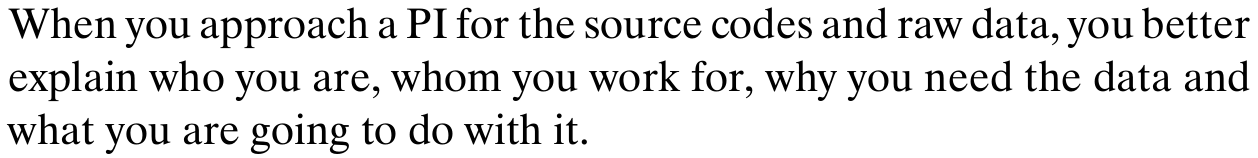
\includegraphics[width=0.95\textwidth]{%
      img/stodden2018_re1.png} %
  \end{figure}

  \begin{figure}
    \centering
    
\includegraphics[width=0.95\textwidth]{%
      img/stodden2018_re2.png} %
  \end{figure}

  \begin{figure}
    \centering
    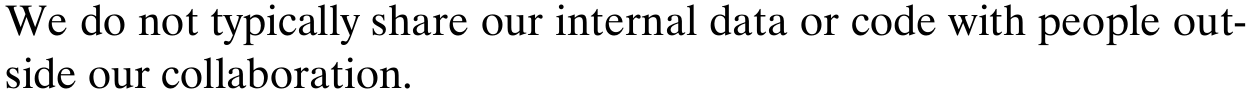
\includegraphics[width=0.95\textwidth]{%
      img/stodden2018_re3.png} %
  \end{figure}

  \source{\cite{Stodden2018}}
  
\end{frame}

\begin{frame}{But also...}
  
  \begin{figure}
    \centering
    
\includegraphics[width=0.95\textwidth]{%
      img/stodden2018_re4.png} %
  \end{figure}

  \begin{figure}
    \centering
    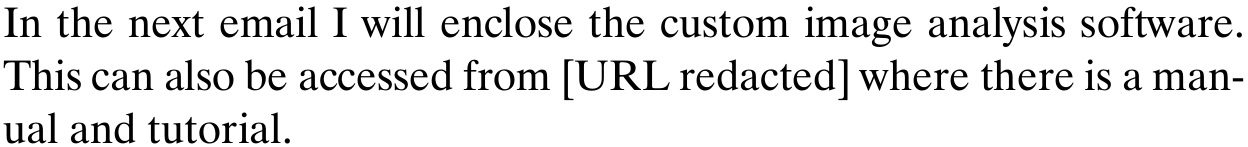
\includegraphics[width=0.95\textwidth]{%
      img/stodden2018_re5.png} %
  \end{figure}

  \begin{figure}
    \centering
    
\includegraphics[width=0.95\textwidth]{%
      img/stodden2018_re6.png} %
  \end{figure}

  \source{\cite{Stodden2018}}
  
\end{frame}


\begin{frame}{\large   Of $N=206$ articles published in \textit{Science} since 2011...}


  \begin{figure}
    \centering
    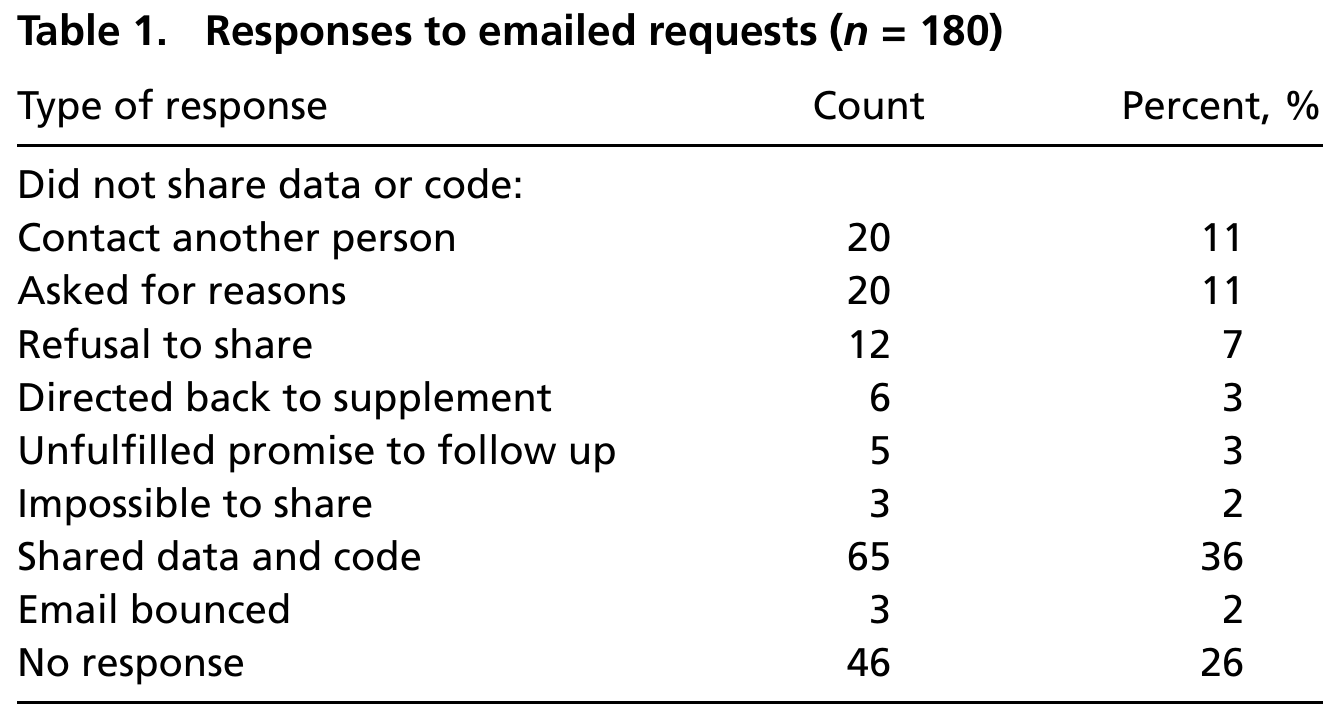
\includegraphics[width=0.95\textwidth]{%
      img/stodden2018_table1.png} %
  \end{figure}
  


  \source{\cite{Stodden2018}}
  
\end{frame}





\begin{frame}{\large Measuring Reproducibility in Computer Systems Research}

  \begin{figure}
    \centering
    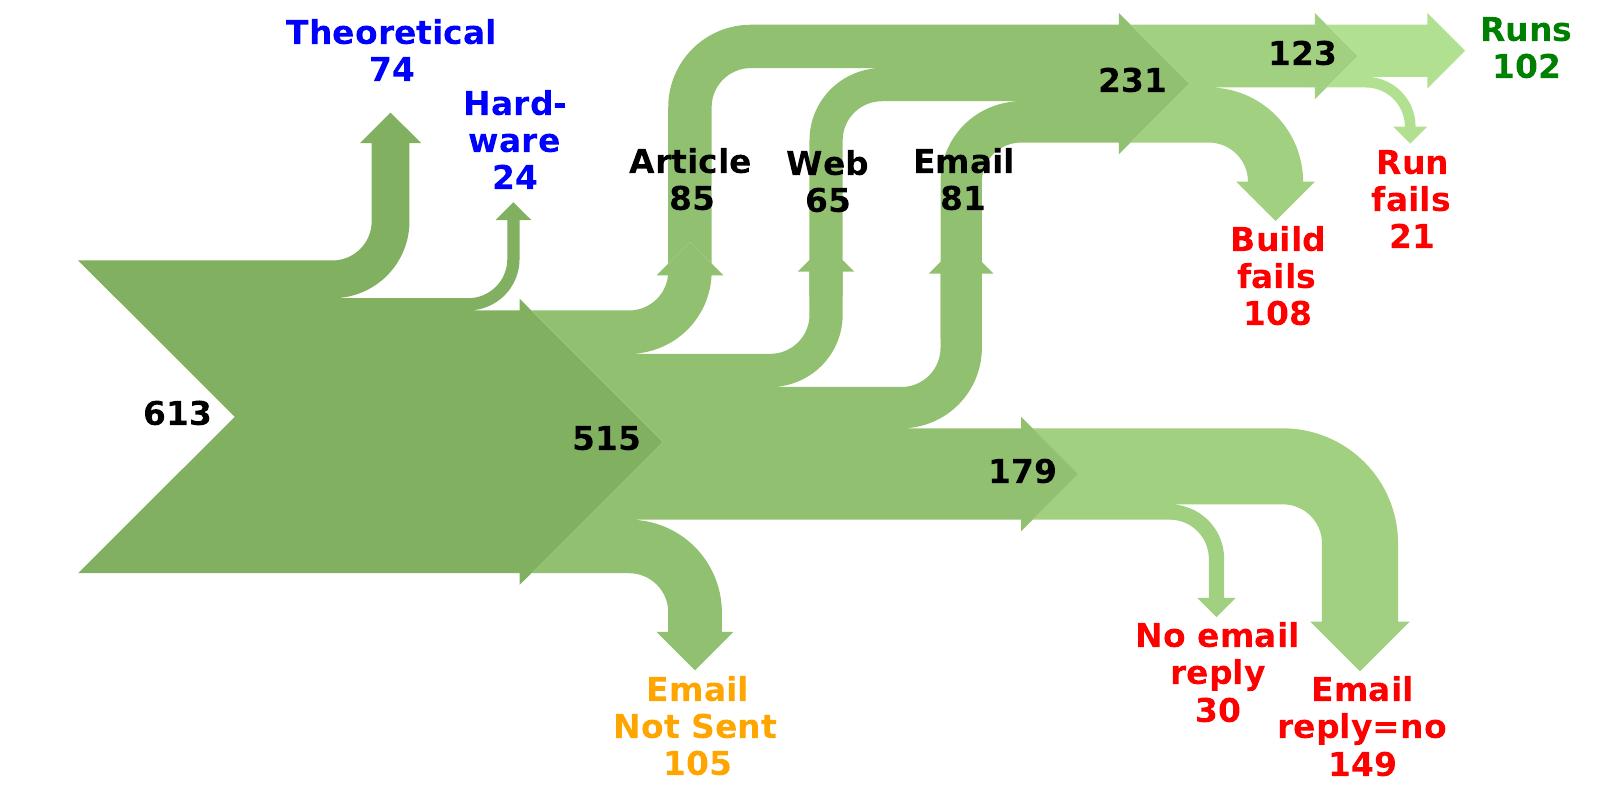
\includegraphics[width=\textwidth]{%
      img/collberg2013_results3.png} %
  \end{figure}
  

  \source{\cite{Collberg2013}}

  \pnote{
    
    613 papers from \\
    - 8 conferences \\
    - 5 journals

    30 minutes of programmer time to try \\
    make build compile/run
    
    Orange: Don't send more than one email to any author \\
    (if author had multiple publications)

    Even if build runs does not even try verify results! \\
    How many more papers will fall off?
    
  }
  
  
\end{frame}


\begin{frame}{\large Why wasn't code available? (Or, the dog ate my program)}
  
  
  
\end{frame}
